\documentclass[a4paper]{article}
\author {Vavilov Andrei}
\title {Animarea modelelor 3D folosind retele neuronale}

\usepackage[utf8]{inputenc}
\usepackage[T1]{fontenc}
\usepackage{textcomp}
\usepackage{amsmath, amssymb}
\usepackage[ht]{graphicx}
% figure support
\usepackage{import}

\pdfminorversion=7
\usepackage{pdfpages}
\usepackage{transparent}
\newcommand{\incfig}[1]{%
	\def\svgwidth{\columnwidth}
	\import{./figures/}{#1.pdf_tex}
}
\setlength{\parskip}{1em}
\pdfsuppresswarningpagegroup=1

\begin{document}

\maketitle

\section{Introducere}
    Inteligenta artificiala este un domeniu foarte versatil, a carui aplicabilitate poate fi extinsa in foarte multe
    domenii,printre care si modelarea grafica, mai exact in modelarea si animarea 3D.


    Urmatorul studiu isi propune sa prezinte o parte din modelele si tehnologiile care pot fi folosite pentru a
anima un model 3D in timp real, pe baza unui fisier audio selectat de catre utilizator.

\section{Tehnologii propuse}
Deoarece inteligenta artificiala este unul dintre cele mai intens cercetate domenii din prezent, exista o varietate de
tehnologii si instrumente pentru realizarea de proiecte.

In continuare voi prezenta si argumenta pe scurt alegerile facute.

\subsection{Limbajul de programare }
O intrebare care a aparut odata cu cresterea in populariate a domeniului inteligentei artificiale este
``Ce limbaj de programare ar trebui sa folosesc?''.Desi nu exista ``cel mai bun limbaj pentru inteligenta artificiala''[ref
la articolulde pe tds], Python este de cele mai multe ori alegerea preferata atat a programatorilor cat si a oamenilor
de stiinta si a statisticienilor datorita:
\begin{enumerate}
	\item Varietatea de framework-uri si instrumente pentru Machine Learning, Data science si modelare/interpretare
		a datelor (TensorFlow, Scipy, Pytorch, Numpy, Pandas).
	\item Numarul mare de resurse disponibile online
	\item Sintaxa simpla
	\item Fiind un limbaj \textit{dinamically typed}, realizarea de aplicatii/modele este facila si rapida.
	\item Fiind un limbaj \textit{cross platform}, aplicatiile sunt automat suportate pe o varietate mare de
		platforme si sisteme de operare.
\end{enumerate}
\subsection{Tipul de \textit{Neural Network} folosit}
Inainte de a argumenta alegerea retelei neuronale, trebuie introdus pe scurt conceptul
de \textbf{\textit{Deep Learning}}.

\textit{Deep Learning}, cunoscut si sub numele de \textit{Deep Structured Learning},
face parte din familia invatarii automate si reprezinta o combinare a algoritmilor de \textit{Machine Learning} cu
\textit{Representation Learning} (tehnica de automatizare a interpretarii datelor). Principalul avantaj pe care
\textit{Deep Learning Neural Networks} il prezinta fata de algoritmii de \textit{Machine Learning} este minimizarea
interventiei factorului uman, prin automatizarea procesului de \textit{feauture extraction}, adica extragerea
caracteristicilor distinctive ale datelor de intrare.


Din categoria \textit{Deep Learning Neural
Networks} trebuie amintite \textbf{ANN, CNN, si RNN}, principalele categorii de \textit{Deep Learning Neural Networks}.
\begin{itemize}


	\item ANN

\begin{figure}[ht]
	\centering
	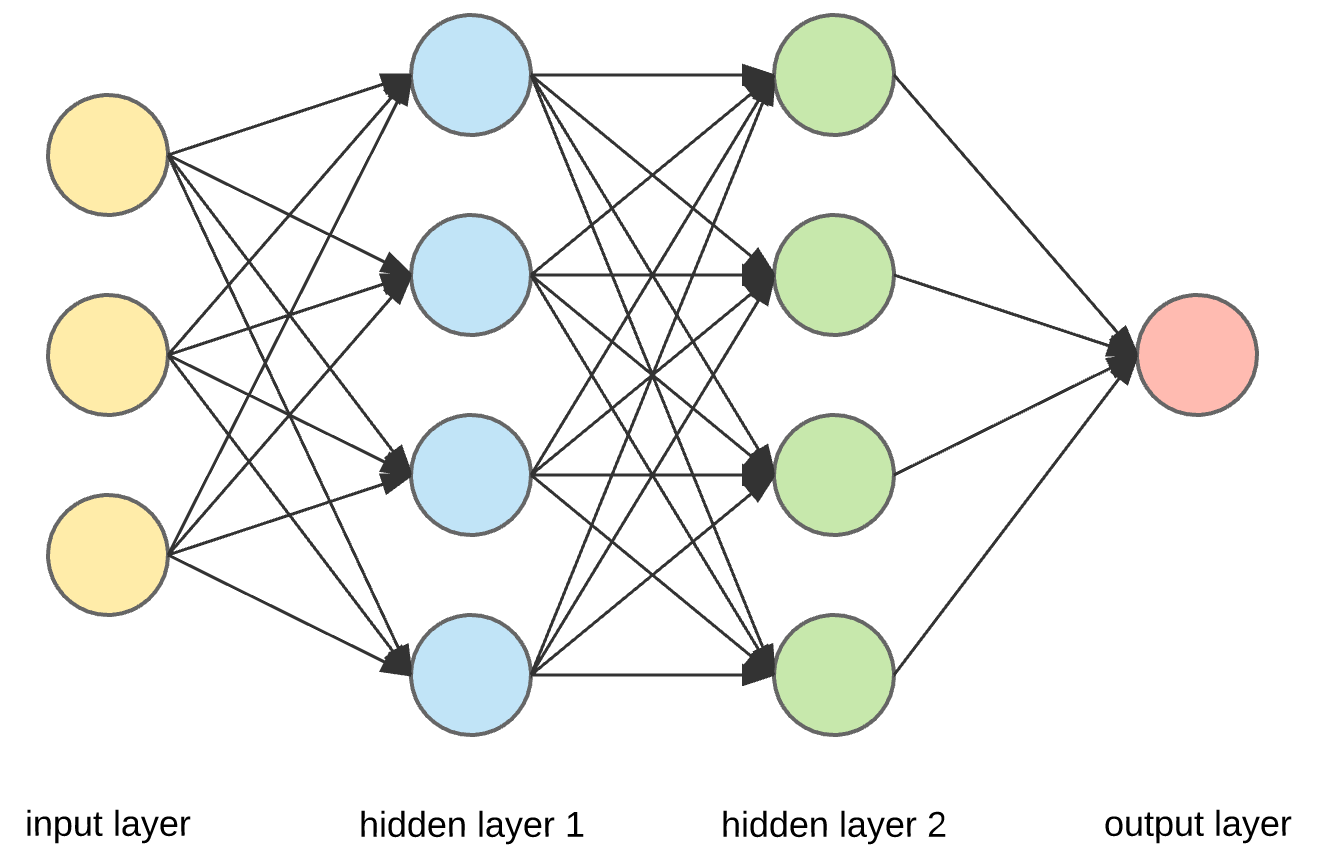
\includegraphics[width = 1.8in]{ann.png}
\label{ANN}
\end{figure}
Retelele neuronale de tip ANN au ca si caracteristica principala prelucrearea unidirectioanla a datelor (\textit{forward feeding})
si este un tip de retea preferata in general in cazul problemelor din spectrul buisness-ului( predictii in legatura cu vanzarile/
viitoarele interese ale cumparatorilor, validare de date, risk management, etc.).

	\item CNN
\begin{figure}[ht]
	\centering
	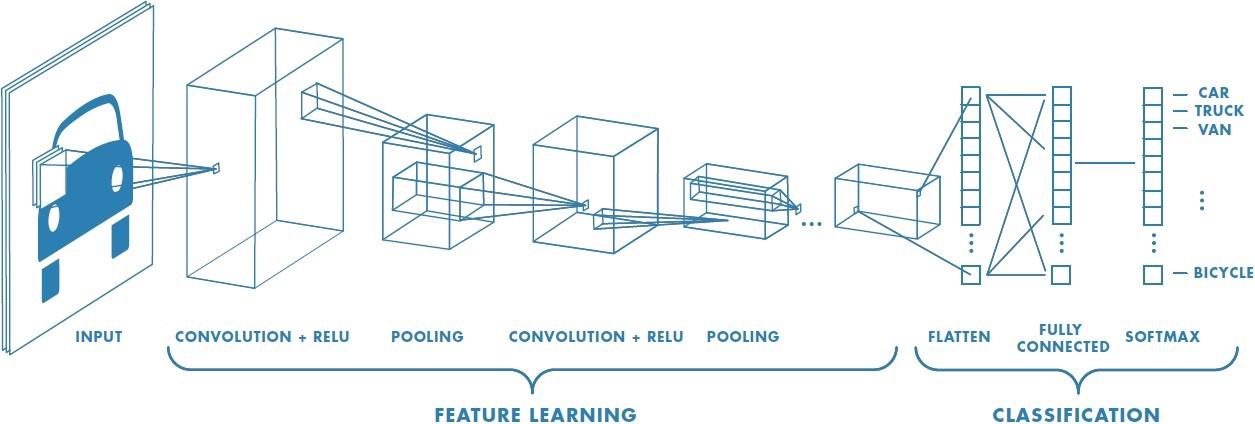
\includegraphics[width = 1.8in]{cnn.jpeg}
\label{CNN}
\end{figure}


Retelele neuronale de tip CNN sunt folosite in cadrul problemelor de clasificare a imaginilor, acestea prelucrand caracteristicile
spatiale(pozitia pixelilor si relatiile dintre acestia).

	\item RNN
Retelele neuronale de tip RNN, desi au o structura relativ asemanatoare cu ANN, se deosebesc prin capacitatea de a prelucra datele
in ambele directii (\textit{recurrent feeding}), fiind astfel o optiune valida preferata in cazul problemelor de procesare text
si audio. RNN transmite secvential informatia catre straturile de neuroni, determinand dependentele dintre componentele datelor
de intrare. Aceasta proprietate distinctiva se numeste \textit{Parameter sharing} si duce la scaderea numarului de neuroni necesari
din retea si, implicit, la scaderea costurilor computationale.
\begin{figure}[ht]
	\centering
	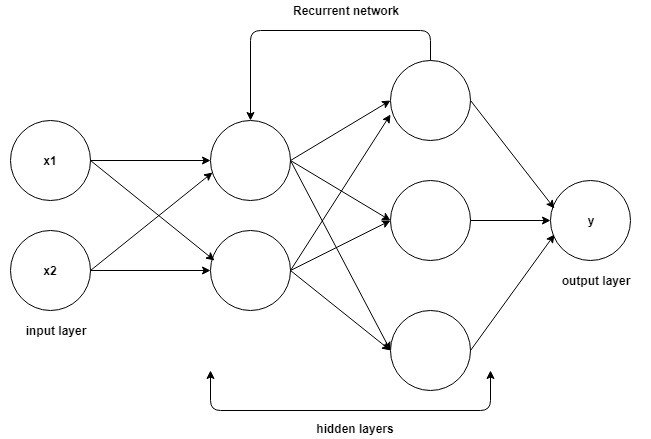
\includegraphics[width = 1.8in]{rnn.jpeg}
\label{RNN}

\end{figure}

\end{itemize}


 \section {Prezentarea tehnologiilor propuse}

\section{Concluzie}

\section{Bibliografie}

\end{document}
